\subsection{Source of Data}
The dataset for this project was obtained from a Kaggle repository titled \textit{Dangerous Heartbeat Dataset (DHD)} \cite{Dangerous-Heartbeat-Dataset-DHD},
which in turn sources its data from the PASCAL Classifying Heart Sounds Challenge 2011 (CHSC2011) \cite{pascal-chsc-2011}.
This dataset comprises audio recordings of heartbeats, categorized into different types of heart sounds.
Specifically, the dataset consists of 5 types of recordings: Normal Heart Sounds, Murmur Sounds, Extra Heart Sounds, Extrasystole Sounds, and Artifacts.
Data has been gathered from the general public via the iStethoscope Pro iPhone app and from a clinic trial in hospitals using the digital stethoscope DigiScope.

\subsubsection*{Type of Sources} %Davide
The dataset comprises audio recordings collected from three distinct sources:
\paragraph{Type A:}
This subset includes recordings contributed by the general public through the iStethoscope Pro iPhone app.
Users from diverse backgrounds and locations have submitted these recordings, providing a wide range of heart sounds in various conditions.
\paragraph{Type B:}
This subset consists of recordings obtained from clinical trials conducted in hospitals using the DigiScope digital stethoscope.
These recordings are collected in controlled environments, contributing to a high-quality dataset for clinical applications.
\paragraph{Type C:}
This subset is a mixed collection that includes recordings from both the iStethoscope Pro app and the DigiScope digital stethoscope.
Additionally, this subset incorporates heart sound recordings sourced from various publicly available datasets on the internet.
This mixed dataset is valuable for its diversity and comprehensiveness, covering a broad spectrum of heart sound variations and abnormalities.

\noindent
These diverse sources ensure a robust dataset that supports comprehensive analysis and improves the generalizability of the heartbeat audio classification model.
\subsubsection*{Classes} % Davide

Heart sounds can be categorized into different classes based on their acoustic characteristics and clinical significance.
Accurate classification of these sounds is essential for diagnosing and treating a variety of cardiac conditions.
The primary categories include Normal heart sounds, Murmurs, Extra Heart Sounds, Artifacts, and Extra Systoles.
Understanding the distinct features and clinical implications of each class is a crucial step before building a
machine learning model to classify heartbeats.
This phase is particularly important for the identification of patterns that are characteristic of specific classes,
which in turn guides the selection of features to extract from the audio.
This knowledge aids in identifying specific patterns and anomalies within the heart sounds,
leading to more precise and reliable model predictions.

\paragraph{Normal}
The Normal category includes recordings of typical, healthy heart sounds. These sounds exhibit the characteristic ``lub-dub, lub-dub'' pattern,
where ``lub'' (S1) represents the closing of the atrioventricular valves and ``dub'' (S2) signifies the closing of the semilunar valves.
In a normal heart, the time interval between ``lub'' and ``dub'' is shorter than the interval from ``dub'' to the next ``lub,''
especially when the heart rate is below 140 beats per minute. Most normal heart rates at rest fall between 60 and 100 beats per minute,
though rates can vary from 40 to 140 beats per minute based on factors such as age and activity level.
Recordings may include background noises like traffic or radio sounds and may capture incidental noises such as breathing or microphone
contact with clothing or skin. It contains both clean and noisy normal recordings,
the latter featuring significant background noise or distortion, which simulates real-world conditions.\\
Figure \ref{fig:normal_heart_beat_audio} shows a sample of a normal heart beat audio.
The characteristic ``lub-dub, lub-dub'' pattern can be observed, where the peaks represent the ``lub'' (S1) and ``dub'' (S2) sounds of a healthy heart.

\begin{figure}[H]
    \centering
    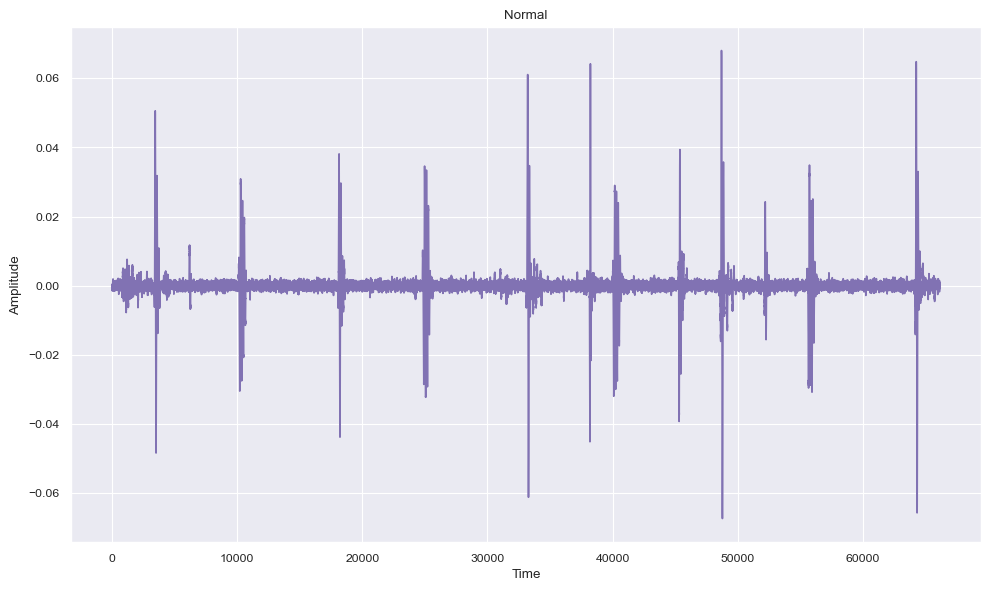
\includegraphics[width=.9\columnwidth]{../images/normal_heart_beat_audio.png}
    \caption{Sample of normal heart beat audio.}
    \label{fig:normal_heart_beat_audio}
\end{figure}

\paragraph{Murmur}
Heart murmurs are abnormal sounds during the heartbeat cycle, such as a ``whooshing, roaring, rumbling, or turbulent fluid'' noise, heard between
the ``lub'' and ``dub'' (systolic murmur) or between ``dub'' and ``lub'' (diastolic murmur).
These murmurs are typically indicative of turbulent blood flow in the heart and can signal various heart conditions, some of which may be serious.
It is crucial to distinguish murmurs from the normal ``lub-dub'' sounds since they occur between the primary heart sounds and not concurrently with them.
It also includes noisy murmur data, which mimics real-world recording scenarios by incorporating significant background noise and distortions.\\
Figure \ref{fig:murmur_heart_beat_audio} shows a sample of a murmur heart beat audio.
The presence of additional sounds between the ``lub'' and ``dub'' peaks can be observed, indicating the characteristic
``whooshing, roaring, rumbling, or turbulent fluid'' noise typical of heart murmurs.

\begin{figure}[H]
    \centering
    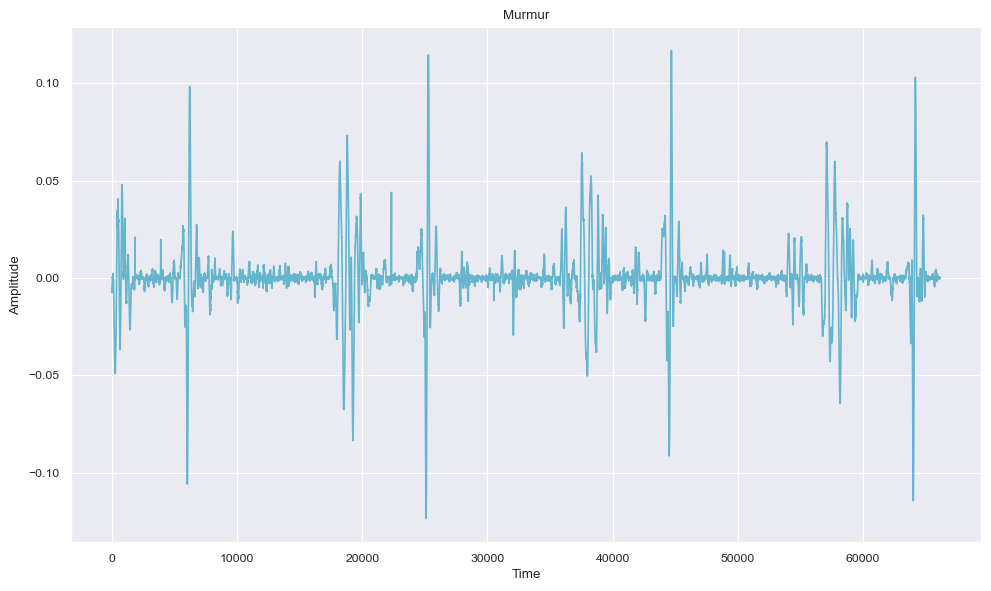
\includegraphics[width=.9\columnwidth]{../images/murmur_heart_beat_audio.png}
    \caption{Sample of murmur heart beat audio.}
    \label{fig:murmur_heart_beat_audio}
\end{figure}

\paragraph{Extra Heart Sound}
Extra heart sounds are characterized by an additional sound in the cardiac cycle, producing patterns such as ``lub-lub dub'' or ``lub dub-dub''.
These sounds can arise from physiological or pathological conditions. For example, a third heart sound (S3) may indicate heart failure or volume overload,
while a fourth heart sound (S4) can be associated with a stiff or hypertrophic ventricle.
Detecting these extra sounds is important for identifying potential heart diseases early, allowing for timely intervention and management.
Figure \ref{fig:extrahls_heart_beat_audio} shows a sample of an extra heart sound audio.
The presence of additional peaks within the normal ``lub-dub'' pattern indicates extra heart sounds, which can be
critical for diagnosing various heart conditions.

\begin{figure}[H]
    \centering
    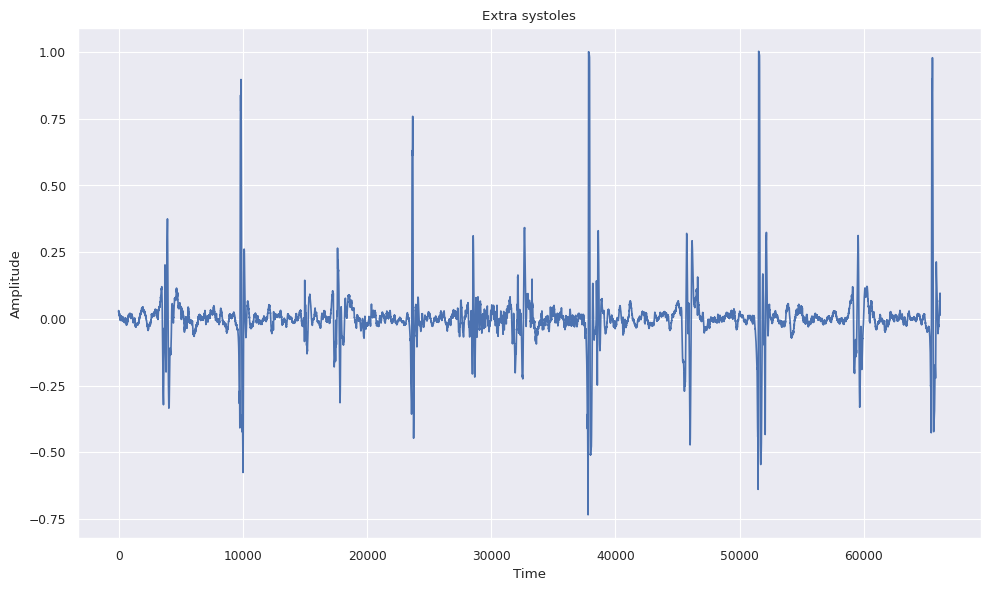
\includegraphics[width=.9\columnwidth]{../images/extrastoles_heart_beat_audio.png}
    \caption{Sample of extra heart sound audio.}
    \label{fig:extrahls_heart_beat_audio}
\end{figure}

\paragraph{Artifact}
The Artifact category consists of recordings with non-cardiac sounds, including feedback squeals, echoes, speech, music, and various types of noise.
These recordings generally lack discernible heart sounds and do not exhibit the temporal periodicity typical of heartbeats at frequencies below 195 Hz.
Accurately identifying artifacts is essential to avoid misinterpreting non-cardiac sounds as pathological heart sounds,
ensuring that data collection efforts focus on genuine heart sounds.
Figure \ref{fig:artifact_heart_beat_audio} shows a sample of an artifact heart beat audio, there can be observed that there is not a clear pattern in the audio.

\begin{figure}[H]
    \centering
    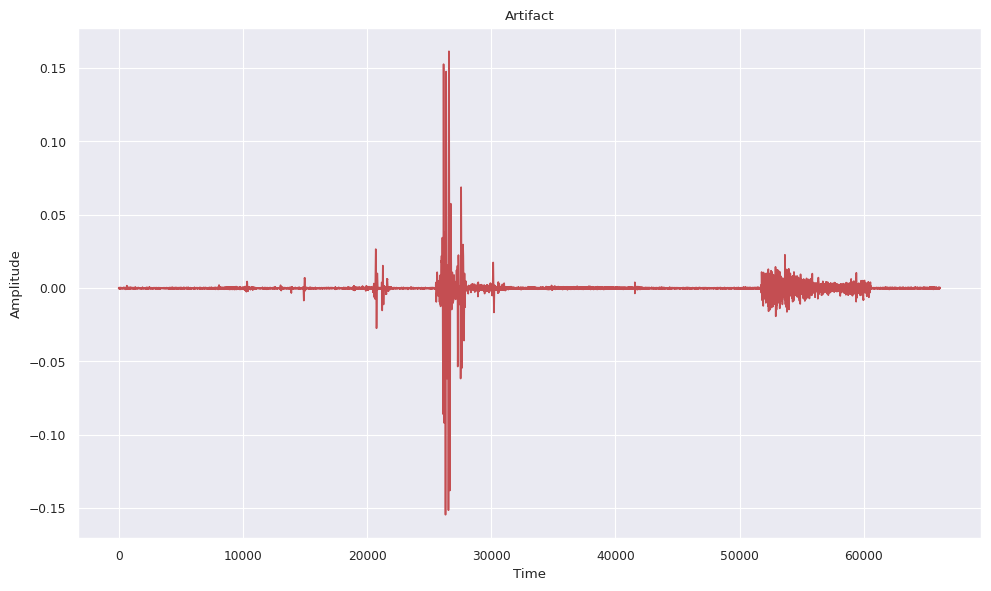
\includegraphics[width=.9\columnwidth]{../images/artifact_heart_beat_audio.png}
    \caption{Sample of artifact heart beat audio }\label{fig:artifact_heart_beat_audio}
\end{figure}

\paragraph{Extra systoles}
Extra systoles refers to extra or skipped heartbeats, resulting in irregular patterns such as ``lub-lub dub'' or ``lub dub-dub''.
Unlike the regular extra heart sounds, extra systoles are sporadic and do not follow a consistent rhythm.
These premature beats can occur in healthy individuals, particularly children, but they may also be associated with various heart diseases.
Identifying extra systoles is crucial as they can be early indicators of cardiac conditions that might require medical attention
if they occur frequently or in certain patterns.\\
In the audio signal depicted in Figure \ref{fig:extrastoles_heart_beat_audio}, irregularities within the normal “lub-dub” pattern are evident.
These irregularities manifest as additional peaks or skipped beats, indicating extra systoles.
\begin{figure}[H]
    \centering
    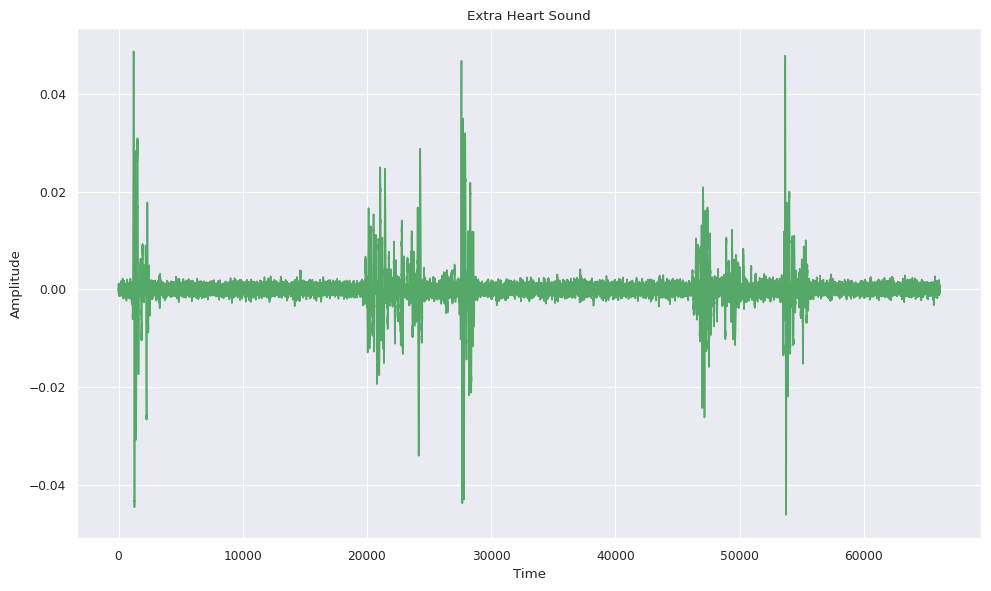
\includegraphics[width=.9\columnwidth]{../images/extrahls_heart_beat_audio.png}
    \caption{Sample of extra systoles heart beat audio }\label{fig:extrastoles_heart_beat_audio}
\end{figure}

\paragraph{Comparison of Heart Sounds}
In Figure \ref{fig:comparison_heart_beat_audio}, a comparison of the different classes of heart sounds can be observed.\\
As we can see, the “Artifact” signal appears erratic with no consistent pattern, likely representing noise or interference rather than true heart sounds.\\
The “Murmurs” signal shows irregular fluctuations in amplitude, which could indicate turbulent blood flow typically associated with murmurs. \\
The signal for “Extra Heart Beat Sound” has occasional spikes in amplitude that stand out from the baseline.\\
The “Normal” signal appears more uniform and regular compared to the others, reflecting the expected rhythm of a healthy heartbeat.
FInally, the signal for “Extra Systoles” shows extra spikes at irregular intervals,
indicating unexpected contractions of the heart muscle (systoles) occurring outside the normal rhythm.

\begin{figure}[H]
    \centering
    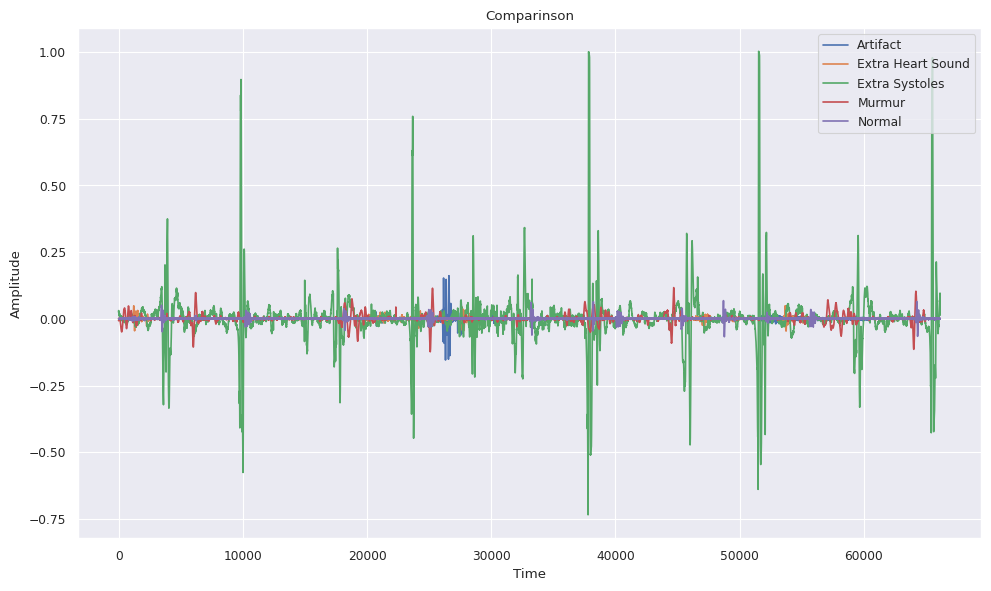
\includegraphics[width=.9\columnwidth]{../images/comparison_heart_beat_audio.png}
    \caption{Comparison of the different classes of heart sounds.}
    \label{fig:comparison_heart_beat_audio}
\end{figure}

\subsubsection*{Data Distribution} % Davide
Figure \ref{fig:DataExp_num_durations}, illustrates the significant class imbalance present in the dataset, particularly for the 'Extrastole' and 'Extrahls' classes,
which have far fewer samples compared to other classes.
This imbalance poses a challenge for the classification task,
as the model may struggle to learn and accurately predict the underrepresented classes due to the insufficient number of training examples.
To mitigate this issue, several strategies are employed.\\
Data augmentation techniques are applied to artificially increase the size of the dataset
by creating modified versions of the existing audio files through methods such as pitch shifting, time stretching, and adding noise.
Additionally, the original audio recordings are segmented into smaller clips, which not only increases the number of samples available for training but
also provides the model with more varied examples of heart sounds, enhancing its ability to generalize across different heart sound variations.\\
Furthermore, the effectiveness of oversampling and undersampling techniques is tested. Oversampling involves duplicating samples from the minority classes
to increase their representation in the training set, while undersampling involves reducing the number of samples from the majority classes
to balance the dataset. The data is split into training and testing sets with an 80\% - 20\% ratio, respectively.\\
A validation set is omitted due to the low number of samples available, ensuring that the maximum amount of data is used for training and testing the model.
\begin{figure}[H]
    \centering
    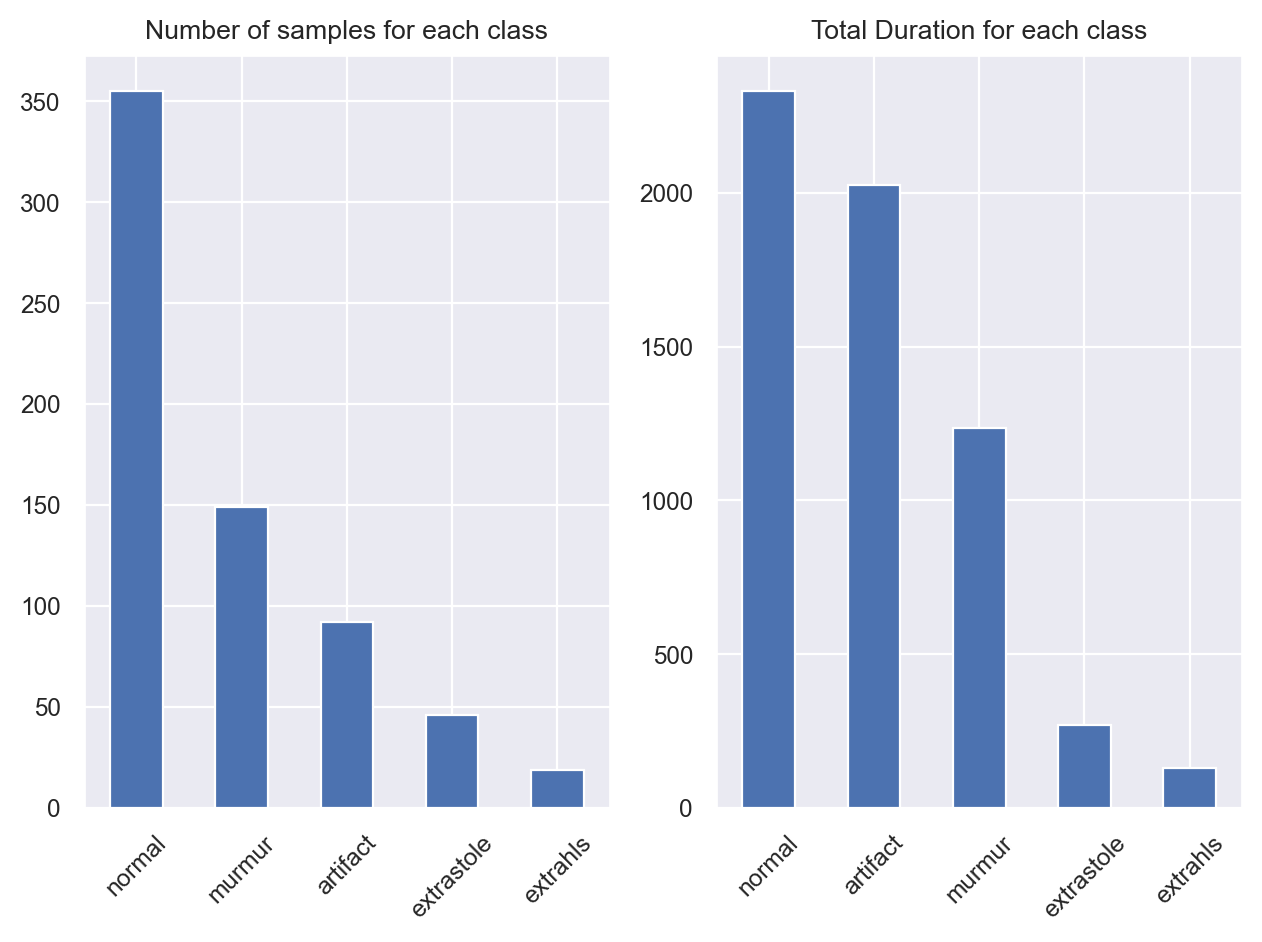
\includegraphics[width=1\columnwidth]{./images/DataExp_num_durations.png}
    \caption{Number of samples per duration.}
    \label{fig:DataExp_num_durations}
\end{figure}

